\documentclass[11pt,a4paper]{article}

\usepackage[T1]{fontenc}
\usepackage[scaled=0.92]{helvet}
\renewcommand{\familydefault}{\sfdefault}
\usepackage{amsmath,amssymb}
\usepackage[margin=2.3cm]{geometry}
\usepackage{booktabs,array,colortbl}
\usepackage{graphicx}
\usepackage{float}
\usepackage[font=small,labelfont=bf]{caption}
\usepackage{enumitem}
\usepackage[colorlinks=true,linkcolor=aimsred,urlcolor=aimsred]{hyperref}
\usepackage{xcolor}

\definecolor{aimsred}{HTML}{990000}
\definecolor{rowpink}{HTML}{F7E9E9}
\definecolor{boxgrey}{HTML}{F4F4F4}

\usepackage{titlesec}
\titleformat{\section}{\Large\bfseries\color{aimsred}}{\thesection}{0.6em}{}
\titleformat{\subsection}{\large\bfseries\color{aimsred}}{\thesubsection}{0.6em}{}
\titleformat{\subsubsection}{\normalsize\bfseries}{\thesubsubsection}{0.6em}{}
\setlist{itemsep=0.25em,topsep=0.4em}
\setlength{\parskip}{0.55em}
\setlength{\parindent}{0pt}

\newcommand{\hl}[1]{{\bfseries\color{aimsred}#1}}
\newcommand{\key}[1]{\par\medskip\noindent\fcolorbox{aimsred}{rowpink}{\parbox{0.94\linewidth}{#1}}\par\medskip}
\newcommand{\R}{\mathcal R_0}

\begin{document}

% ======================================================================
\begin{center}
{\large\color{gray} Training Workshop on Mathematical Biology 2026 \quad|\quad Project 3}\\[0.8em]
{\LARGE\bfseries\color{aimsred} Does the disease survive?}\\[0.4em]
{\Large\bfseries Stochastic versus deterministic models of\\ endemic and multi-strain infections}
\end{center}
\bigskip

% ======================================================================
\section*{Summary}

We compare two ways of modelling the same infection: a \hl{deterministic} model (ordinary differential equations, ODE), in which the number of infected people is a continuous quantity, and a \hl{stochastic} model (Gillespie stochastic simulation algorithm, SSA), in which individuals are counted one by one and every event is random.

\textbf{Part 1: one strain with waning immunity (SIRS).}
The ODE predicts that the infection stays in the population for ever (an \emph{endemic} state) whenever the population size is $N>N_c=\gamma/\beta=15$, with $I^*=\frac{\omega}{\omega+\gamma}\big(N-\frac{\gamma}{\beta}\big)$ infected people. The SSA disagrees for small populations: out of 500 runs, \emph{none} is still infected after one year for $N\le 40$, 7\% for $N=70$ and 56\% for $N=100$. When the infection does survive, its mean level agrees with the ODE.

\textbf{Part 2: two competing strains with waning immunity, births, deaths and cross infection.}
\begin{itemize}
  \item Both strains can spread: $\R^1=2.31$, $\R^2=3.84$. The disease free state is unstable.
  \item The ODE settles on a \hl{stable coexistence} of both strains ($I_1^*=0.103$, $I_2^*=0.211$), reached through damped oscillations that fade within about a year. There are no sustained cycles.
  \item Coexistence is explained by \emph{mutual invasibility}: each strain can invade a population where the other is endemic (invasion numbers $3.83$ and $2.27$, both above 1), because people recovered from one strain are still susceptible to the other.
  \item With $N=10{,}000$ people the SSA fluctuates around the ODE levels and no strain is lost in 50 years.
  \item In the ODE an infected fraction can never reach zero, so a strain can drop to a tiny value and rebound. In the SSA zero is \hl{absorbing}: when the count of a strain reaches 0, the strain is gone for ever. With $k$ infected people a strain is lost with probability about $(1/\R)^k$, so a \hl{bottleneck} (few carriers at the lowest point of the trajectory) decides survival. For small populations both strains are lost, although the ODE predicts coexistence for every $N$: 100\% of runs at $N\le 200$, 60\% at $N=400$, 8\% at $N=700$, 2\% at $N=1000$.
\end{itemize}

\key{\textbf{Main message.} The ODE describes the large population limit and says what is \emph{possible}. The stochastic model says what \emph{happens} in a finite population. Threshold conditions such as $N>\gamma/\beta$ or $\R>1$ are necessary for persistence, not sufficient.}

% ======================================================================
\section{Background: the two modelling approaches}

Both models are built from the same list of \emph{events}. Each event changes the state by a fixed vector and happens at a rate (its \emph{propensity}).

\begin{center}
\renewcommand{\arraystretch}{1.4}
\begin{tabular}{p{2.8cm}p{5.6cm}p{6.2cm}}
\rowcolor{aimsred}\color{white}& \color{white}ODE (deterministic) & \color{white}Gillespie SSA (stochastic)\\
Counts are & continuous numbers & whole numbers of people\\
\rowcolor{rowpink}Result & one smooth curve & a random path, different in every run\\
Can reach zero? & never (shown in Section~\ref{sec:zero}) & yes, and then it is final\\
\rowcolor{rowpink}Describes & the average, for large numbers & exact sample paths of the process
\end{tabular}
\end{center}

\textbf{Gillespie direct method.} In a state $\mathbf x$ with propensities $a_1(\mathbf x),\dots,a_M(\mathbf x)$ and total $a_0=\sum_j a_j$:
\begin{enumerate}
  \item draw the waiting time $\tau=-\ln(r_1)/a_0$, with $r_1$ uniform on $(0,1)$ (an exponential with rate $a_0$);
  \item choose event $j$ with probability $a_j/a_0$ (use a second uniform number $r_2$);
  \item update $\mathbf x\to\mathbf x+\boldsymbol\nu_j$ and $t\to t+\tau$; repeat until the final time, or until $a_0=0$.
\end{enumerate}
The ODE is obtained by adding, for every event, its propensity times its state change vector: $\dot{\mathbf x}=\sum_j \boldsymbol\nu_j\,a_j(\mathbf x)$.

\key{\textbf{Why zero matters.} If an event that creates an infection has a propensity proportional to the number of infected people, then at 0 infected people its propensity is 0: nothing can ever restart the infection.}

% ======================================================================
\section{Part 1: one strain with waning immunity (SIRS)}

\subsection{Model}

Three classes $S,I,R$ with $N=S+I+R$ fixed (no births or deaths). Recovered people lose their immunity at rate $\omega$ and return to $S$.

\begin{figure}[H]
\centering
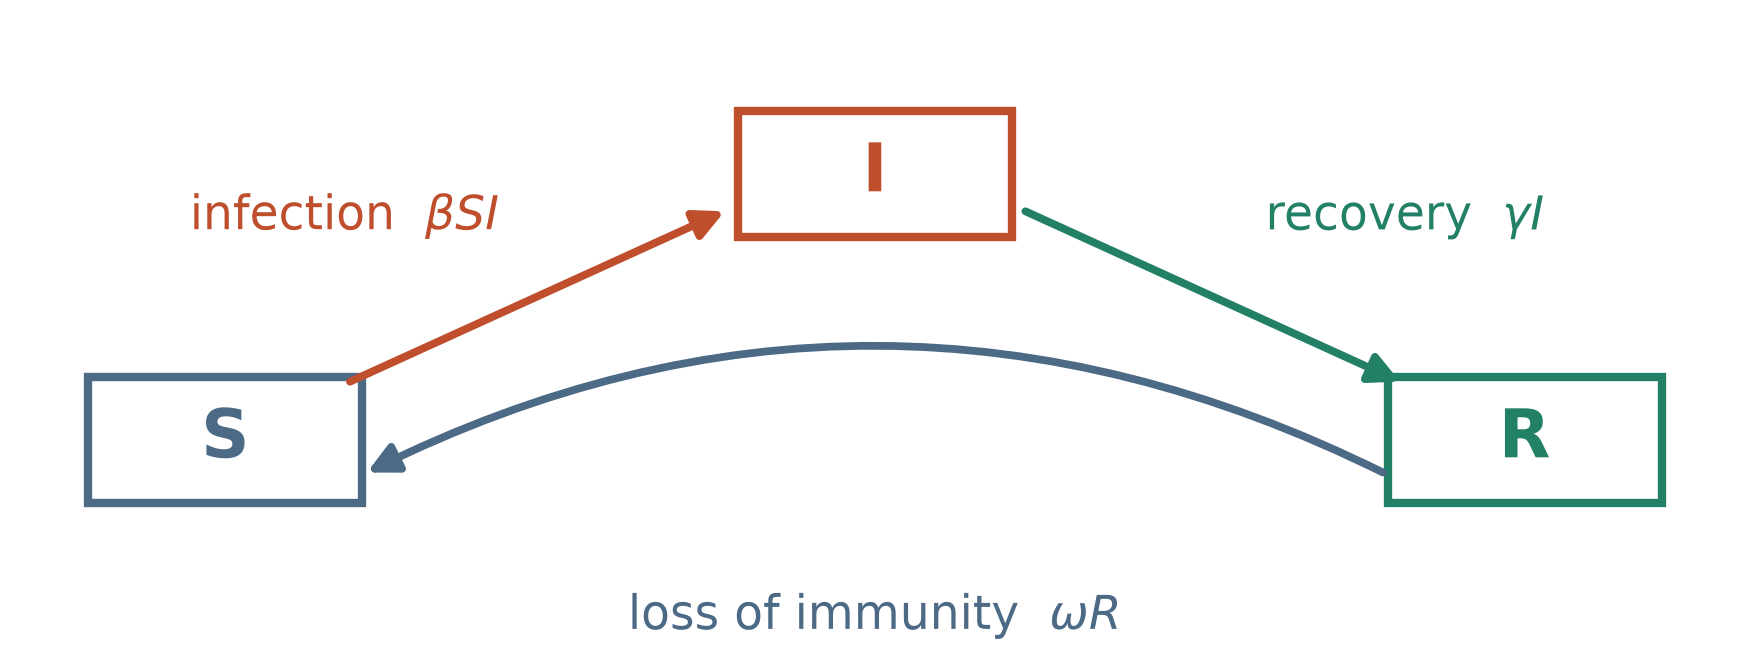
\includegraphics[width=0.62\textwidth]{img/slide_p1_cartoon.png}
\caption{SIRS model. The new event is the loss of immunity $R\to S$, which closes the loop $S\to I\to R\to S$.}
\end{figure}

\begin{center}
\renewcommand{\arraystretch}{1.3}
\begin{tabular}{lccc}
\rowcolor{aimsred}\color{white}Event & \color{white}Reaction & \color{white}Change $[\Delta S,\Delta I,\Delta R]$ & \color{white}Propensity\\
Infection & $S+I\to 2I$ & $[-1,+1,0]$ & $\beta SI$\\
\rowcolor{rowpink}Recovery & $I\to R$ & $[0,-1,+1]$ & $\gamma I$\\
Loss of immunity & $R\to S$ & $[+1,0,-1]$ & $\omega R$
\end{tabular}
\end{center}

Adding the events gives the ODE
\[
\dot S=-\beta SI+\omega R,\qquad \dot I=\beta SI-\gamma I,\qquad \dot R=\gamma I-\omega R .
\]
The three right hand sides add up to zero, so $S+I+R=N$ is constant.

\subsection{Equilibria and the critical population size}

Set every derivative to zero. From $\dot R=0$: $R^*=\frac{\gamma}{\omega}I^*$. From $\dot I=I^*(\beta S^*-\gamma)=0$ there are two cases.

\begin{itemize}
  \item \textbf{Disease free:} $I^*=0$, $R^*=0$, $S^*=N$. It always exists.
  \item \textbf{Endemic:} $S^*=\gamma/\beta$. Then $N=S^*+I^*+R^*=\frac{\gamma}{\beta}+I^*\big(1+\frac{\gamma}{\omega}\big)$, so
  \[
  I^*=\frac{\omega}{\omega+\gamma}\Big(N-\frac{\gamma}{\beta}\Big),\qquad R^*=\frac{\gamma}{\omega+\gamma}\Big(N-\frac{\gamma}{\beta}\Big).
  \]
\end{itemize}
The endemic equilibrium is positive exactly when $N>N_c=\gamma/\beta$, that is when $\R=\beta N/\gamma>1$.

\textbf{Stability.} Eliminate $R=N-S-I$. The Jacobian of $(S,I)$ at the endemic point has trace $-(\beta I^*+\omega)<0$ and determinant $\beta I^*(\beta S^*+\omega)>0$, so it is stable whenever it exists. Parameters of the project (per day): $\beta=0.01$, $\gamma=0.15$ (infectious period about 7 days), $\omega=0.025$ (immunity about 40 days), so $N_c=15$. For $N\ge16$, the ODE solutions over 3000 days reproduce $I^*$ to four decimals (for example $12.1429$ at $N=100$).

\subsection{Stochastic simulation}

Start with one infected person, $(S_0,I_0,R_0)=(N-1,1,0)$; simulate one year; 500 runs for each $N$ between 10 and 100. A run stops if $I=0$, which is absorbing.

\begin{table}[H]
\centering\small
\renewcommand{\arraystretch}{1.2}
\begin{tabular}{rrrrrr}
\rowcolor{aimsred}\color{white}$N$ & \color{white}$\R$ & \color{white}$I^*$ (ODE) & \color{white}fraction of runs infected at day 365 & \color{white}median fade out (days) & \color{white}mean $I$ of survivors\\
10 & 0.67 & 0 & 0.00 & 5.5 & --\\
\rowcolor{rowpink}15 & 1.00 & 0 & 0.00 & 5.9 & --\\
20 & 1.33 & 0.71 & 0.00 & 6.1 & --\\
\rowcolor{rowpink}25 & 1.67 & 1.43 & 0.00 & 10.1 & --\\
30 & 2.00 & 2.14 & 0.00 & 11.5 & --\\
\rowcolor{rowpink}40 & 2.67 & 3.57 & 0.00 & 42.2 & --\\
50 & 3.33 & 5.00 & 0.002 (1 of 500) & 48.1 & 5.12\\
\rowcolor{rowpink}70 & 4.67 & 7.86 & 0.07 & 64.5 & 8.00\\
100 & 6.67 & 12.14 & 0.56 & 99.7 & 11.99
\end{tabular}
\caption{Part 1, results over 500 runs per $N$ (mean $I$ is averaged over days 100 to 365).}
\end{table}

\begin{figure}[H]
\centering
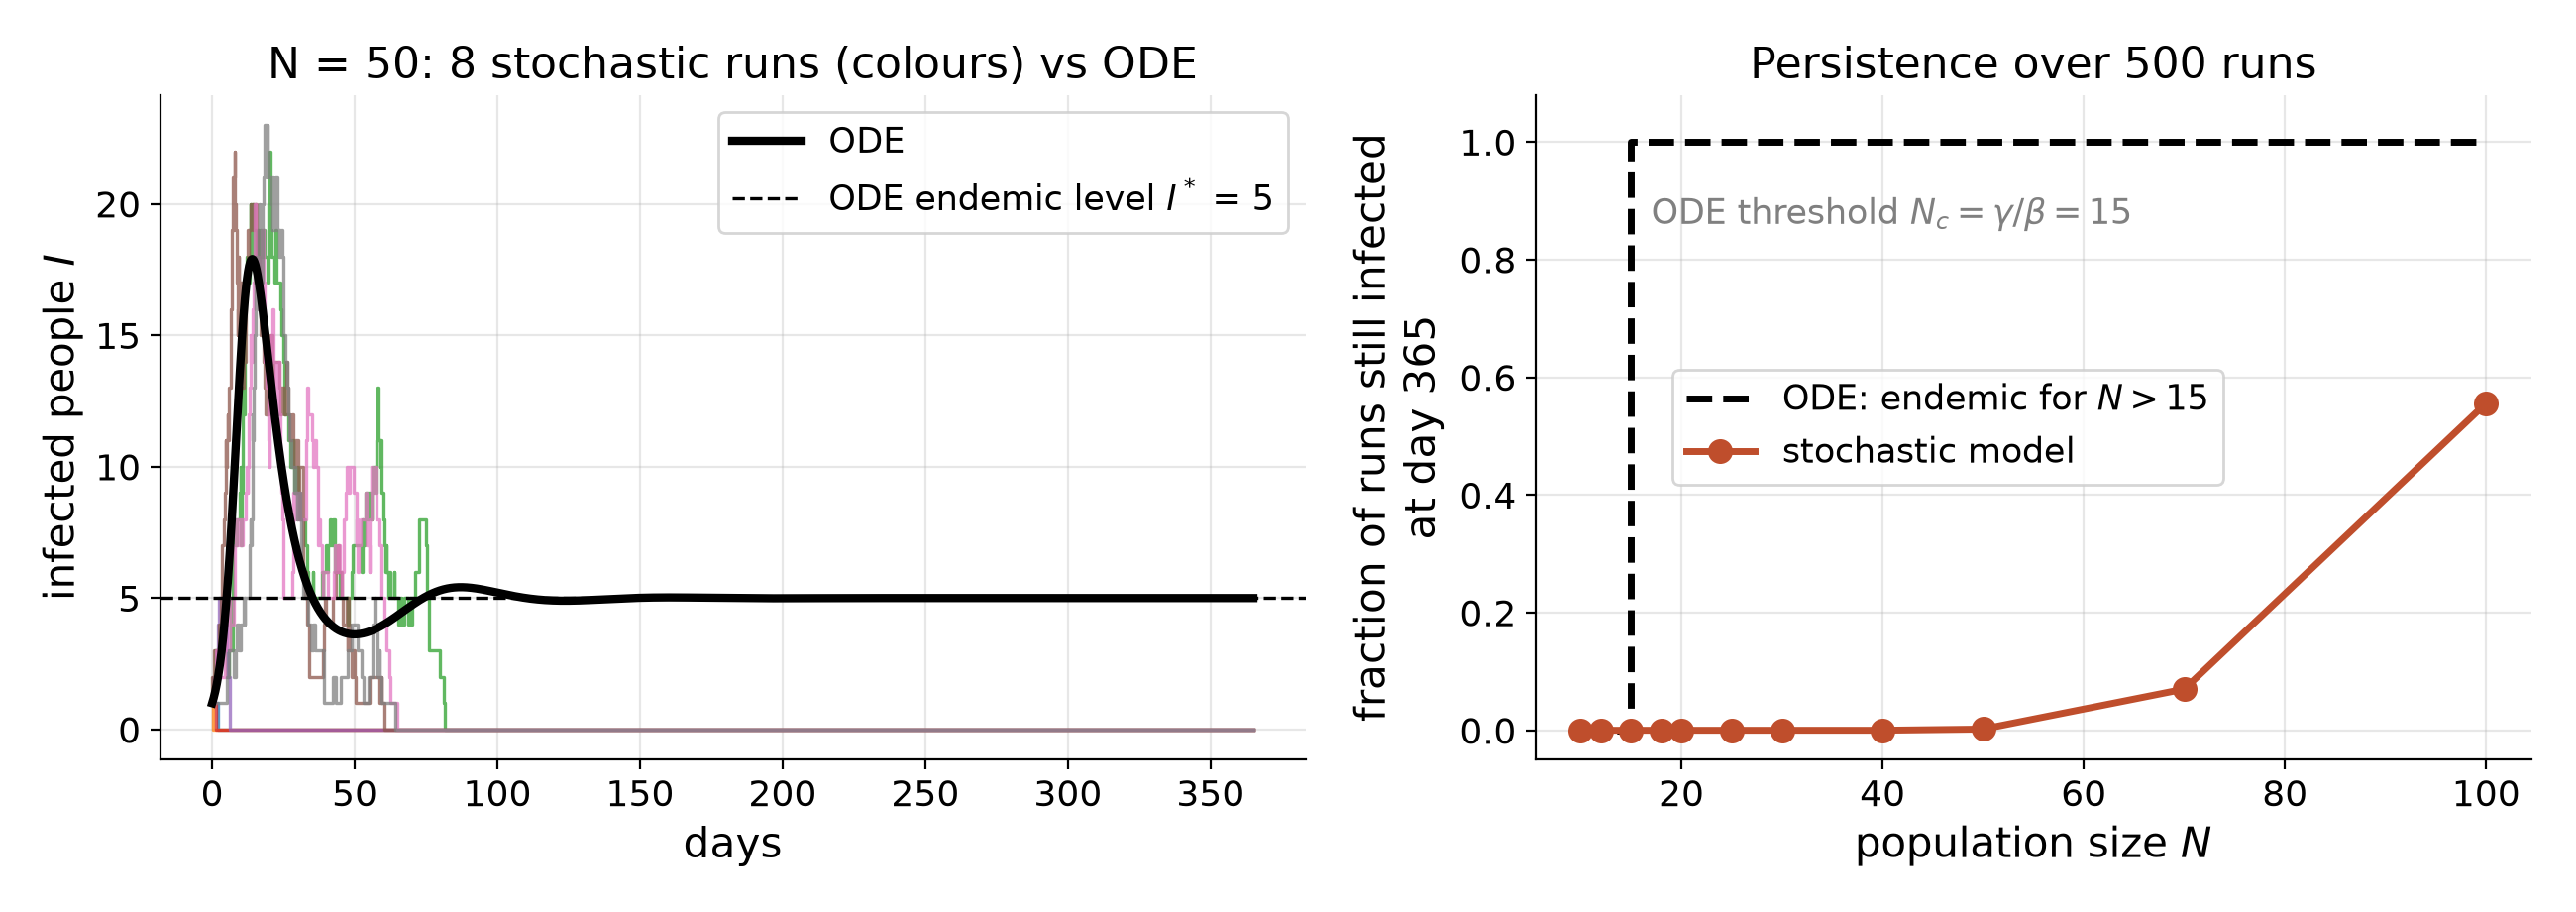
\includegraphics[width=\textwidth]{img/slide_p1_persistence.png}
\caption{Left: $N=50$. The ODE settles at $I^*=5$; all 8 stochastic runs shown reach zero within about three months. Right: fraction of runs still infected after one year. The ODE predicts persistence for every $N>15$.}
\end{figure}

\subsection{Findings}

\begin{itemize}
  \item \textbf{Does the SSA always give an endemic state when the ODE does?} No. For $N$ from 18 to 40 no run out of 500 was infected at day 365, and only 1 of 500 at $N=50$. The two models agree only where the ODE itself predicts extinction ($N\le 15$).
  \item \textbf{Why?} The first epidemic wave leaves few infected people. For small $N$ the equilibrium $I^*$ is only a few people (below one person for $N\le 20$) and fluctuations bring the count to zero, which is final.
  \item \textbf{When the infection survives}, its mean level agrees with the ODE: $5.1$ against $5.0$ at $N=50$, $8.0$ against $7.9$ at $N=70$, $12.0$ against $12.1$ at $N=100$.
\end{itemize}
So $N>N_c$ is necessary for persistence, but not sufficient in a small population.

% ======================================================================
\section{Part 2: two strains with waning immunity}

\subsection{Model and choice of equations}

Five classes: $S$ (susceptible), $I_1,I_2$ (infected with strain 1 or 2), $R_1,R_2$ (recovered from strain 1 or 2). Newborns enter $S$; every class loses people by death at rate $\mu$; immunity wanes from $R_i$ back to $S$. Someone recovered from one strain is still susceptible to the other (\emph{cross infection}). In proportions ($S+I_1+I_2+R_1+R_2=1$):
\begin{align}
\dot S&=\mu(1-S)-\beta_1SI_1-\beta_2SI_2+\omega_1R_1+\omega_2R_2\\
\dot I_1&=\beta_1(S+R_2)I_1-(\gamma_1+\mu)I_1\\
\dot I_2&=\beta_2(S+R_1)I_2-(\gamma_2+\mu)I_2\\
\dot R_1&=\gamma_1I_1-\beta_2R_1I_2-(\omega_1+\mu)R_1\\
\dot R_2&=\gamma_2I_2-\beta_1R_2I_1-(\omega_2+\mu)R_2
\end{align}

\begin{figure}[H]
\centering
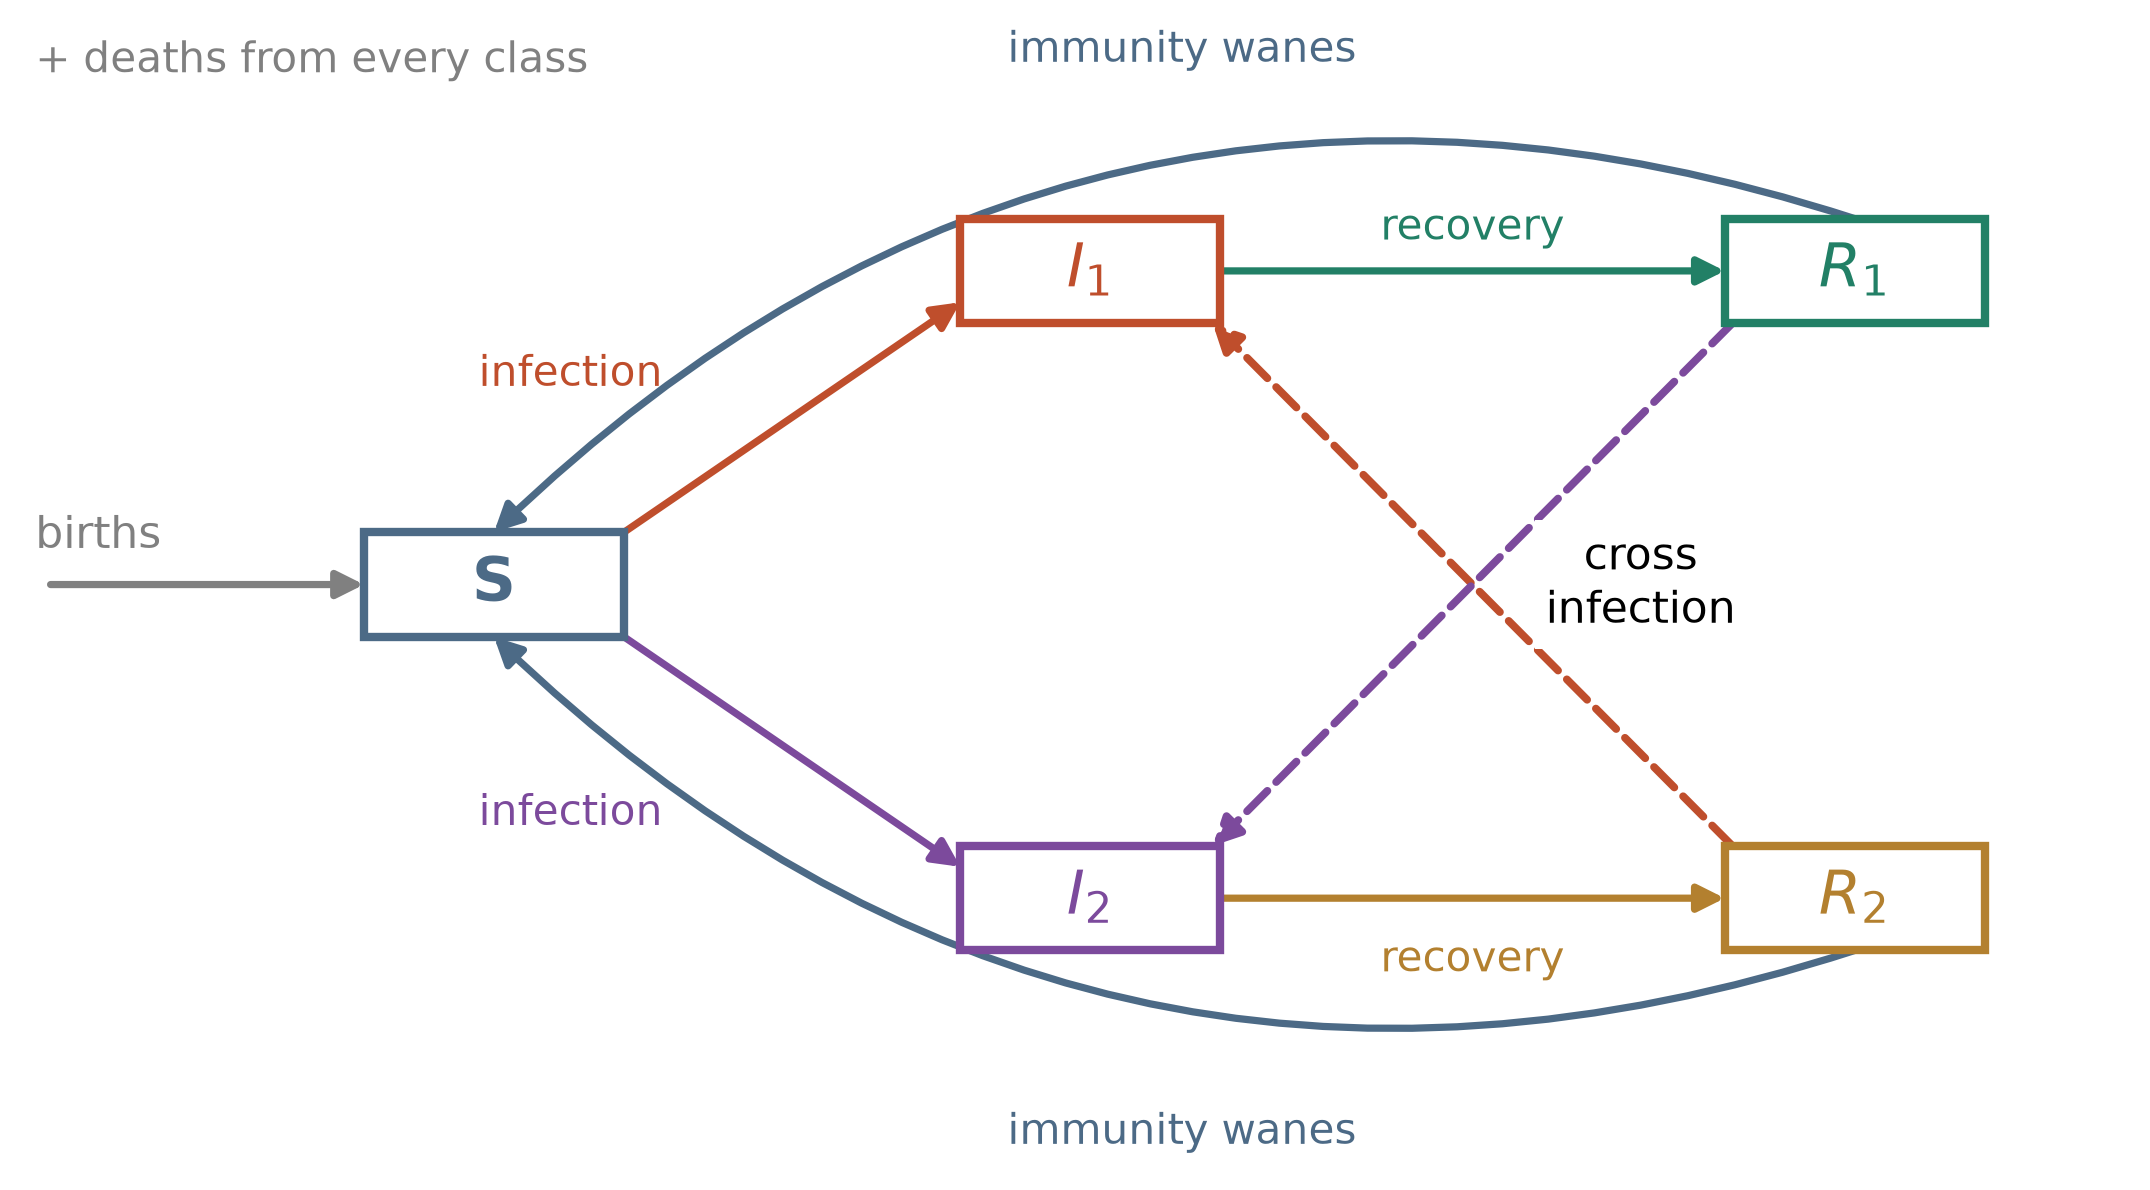
\includegraphics[width=0.72\textwidth]{img/slide_p2_cartoon.png}
\caption{Two strain model. Solid arrows: infection, recovery and waning for each strain. Dashed arrows: cross infection ($R_2\to I_1$ and $R_1\to I_2$). Births enter $S$; deaths leave every class.}
\end{figure}

\textbf{Remarks on the project sheet.}
\begin{enumerate}
  \item The text says ``$\beta_1$ and $\beta_1$''; it must be $\beta_1$ and $\beta_2$.
  \item The equations (2.2) to (2.5) printed in the sheet do not contain the cross infection terms $\beta_1R_2I_1$ and $\beta_2R_1I_2$, but the sheet's text ($R_1$ is susceptible to strain 2 and $R_2$ to strain 1), the sheet's code and its 14 SSA events do. We use the \hl{full model with cross infection} above. The printed version is analysed as a variant in Section~\ref{sec:printed}.
  \item The ODE is in proportions, so in the SSA infections have propensity $\beta SI/N$. This is the same model as in Part 1 with $\beta_{\rm counts}=\beta/N$.
\end{enumerate}

\textbf{Parameters} (time unit: years): $\mu=0.02$, $N=10{,}000$, 50 years, initial state $[S,I_1,I_2,R_1,R_2]=[0.99,0.005,0.005,0,0]$ (counts $[9900,50,50,0,0]$).

\begin{center}
\renewcommand{\arraystretch}{1.3}
\begin{tabular}{lcccc}
\rowcolor{aimsred}\color{white}& \color{white}$\beta$ & \color{white}$\gamma$ & \color{white}$\omega$ & \color{white}meaning\\
Strain 1 & 120 & 52 & 0.2 & infectious 1 week, immunity 5 years\\
\rowcolor{rowpink}Strain 2 & 100 & 26 & 0.5 & infectious 2 weeks, immunity 2 years
\end{tabular}
\end{center}

\subsection{The events of the SSA}

State $[S,I_1,I_2,R_1,R_2]$ in counts. There is one event for each term of the ODE.

\begin{center}
\small\renewcommand{\arraystretch}{1.18}
\begin{tabular}{r l l l}
\rowcolor{aimsred}\color{white}\# & \color{white}Event & \color{white}Change & \color{white}Propensity\\
0 & Birth into $S$ & $[+1,0,0,0,0]$ & $\mu N$\\
\rowcolor{rowpink}1--5 & Death of $S,I_1,I_2,R_1,R_2$ & $-1$ in that class & $\mu S,\mu I_1,\mu I_2,\mu R_1,\mu R_2$\\
6 & $S\to I_1$ & $[-1,+1,0,0,0]$ & $\beta_1SI_1/N$\\
\rowcolor{rowpink}7 & $S\to I_2$ & $[-1,0,+1,0,0]$ & $\beta_2SI_2/N$\\
8 & $R_2\to I_1$ & $[0,+1,0,0,-1]$ & $\beta_1R_2I_1/N$\\
\rowcolor{rowpink}9 & $R_1\to I_2$ & $[0,0,+1,-1,0]$ & $\beta_2R_1I_2/N$\\
10 & $I_1\to R_1$ & $[0,-1,0,+1,0]$ & $\gamma_1I_1$\\
\rowcolor{rowpink}11 & $I_2\to R_2$ & $[0,0,-1,0,+1]$ & $\gamma_2I_2$\\
12 & $R_1\to S$ (waning) & $[+1,0,0,-1,0]$ & $\omega_1R_1$\\
\rowcolor{rowpink}13 & $R_2\to S$ (waning) & $[+1,0,0,0,-1]$ & $\omega_2R_2$
\end{tabular}
\end{center}

\subsection{Reduction to a four dimensional system}\label{sec:reduction}

\textbf{Step 1: the five fractions always add up to 1.} Add the five equations. Every transfer between classes appears once with a plus sign and once with a minus sign:
\begin{itemize}
  \item infection $\beta_1SI_1$: $-$ in $\dot S$, $+$ in $\dot I_1$; infection $\beta_2SI_2$: $-$ in $\dot S$, $+$ in $\dot I_2$;
  \item cross infection $\beta_1R_2I_1$: $+$ in $\dot I_1$, $-$ in $\dot R_2$; cross infection $\beta_2R_1I_2$: $+$ in $\dot I_2$, $-$ in $\dot R_1$;
  \item recovery $\gamma_iI_i$: $-$ in $\dot I_i$, $+$ in $\dot R_i$;
  \item waning $\omega_iR_i$: $+$ in $\dot S$, $-$ in $\dot R_i$.
\end{itemize}
All these terms cancel. What remains is births minus deaths:
\[
\frac{d}{dt}(S+I_1+I_2+R_1+R_2)=\mu-\mu(S+I_1+I_2+R_1+R_2)=\mu\big[1-(S+I_1+I_2+R_1+R_2)\big].
\]
At $t=0$ the sum is $0.99+0.005+0.005=1$, so the right hand side is $0$ and the sum stays 1 for ever (any deviation from 1 would decay like $e^{-\mu t}$). Hence
\[
\boxed{S=1-I_1-I_2-R_1-R_2.}
\]

\textbf{Step 2: substitute in the infected equations.} Factor out $I_1$:
\[
\dot I_1=\beta_1(S+R_2)I_1-(\gamma_1+\mu)I_1,\qquad
S+R_2=(1-I_1-I_2-R_1-R_2)+R_2=1-I_1-I_2-R_1 .
\]
The $R_2$ cancels. In the same way $S+R_1=1-I_1-I_2-R_2$.

\textbf{Step 3: the other equations.} $\dot R_1$ and $\dot R_2$ do not contain $S$, and the equation for $\dot S$ is redundant: on the constraint, $\dot S=-(\dot I_1+\dot I_2+\dot R_1+\dot R_2)$.

\textbf{Result:}
\[
\boxed{\begin{aligned}
\dot I_1&=\beta_1(1-I_1-I_2-R_1)I_1-(\gamma_1+\mu)I_1\\
\dot I_2&=\beta_2(1-I_1-I_2-R_2)I_2-(\gamma_2+\mu)I_2\\
\dot R_1&=\gamma_1I_1-\beta_2R_1I_2-(\omega_1+\mu)R_1\\
\dot R_2&=\gamma_2I_2-\beta_1R_2I_1-(\omega_2+\mu)R_2
\end{aligned}}
\]
The people susceptible to strain 1 are everyone except those infected (with either strain) or protected against strain 1 ($R_1$). People in $R_2$ remain susceptible to strain 1. A symbolic computation confirms all three steps (the differences are identically zero).

\subsection{Disease free equilibrium and basic reproduction numbers}

\textbf{Disease free equilibrium (DFE).} Put $I_1=I_2=0$. Then $\dot R_1=-(\omega_1+\mu)R_1=0$ gives $R_1^*=0$ and likewise $R_2^*=0$, and $\dot S=\mu(1-S)=0$ gives $S^*=1$:
\[
E_0=(S^*,I_1^*,I_2^*,R_1^*,R_2^*)=(1,0,0,0,0).
\]

\textbf{Next generation matrix.} The infected compartments are $x=(I_1,I_2)$. Split $\dot x=\mathcal F-\mathcal V$ with $\mathcal F$ the rate of new infections and $\mathcal V$ the other transfers:
\[
\mathcal F=\begin{pmatrix}\beta_1(S+R_2)I_1\\ \beta_2(S+R_1)I_2\end{pmatrix},\qquad
\mathcal V=\begin{pmatrix}(\gamma_1+\mu)I_1\\ (\gamma_2+\mu)I_2\end{pmatrix}.
\]
At $E_0$ (where $S+R_2=S+R_1=1$) the Jacobians with respect to $(I_1,I_2)$ are
\[
F=\begin{pmatrix}\beta_1&0\\0&\beta_2\end{pmatrix},\quad
V=\begin{pmatrix}\gamma_1+\mu&0\\0&\gamma_2+\mu\end{pmatrix},\quad
K=FV^{-1}=\begin{pmatrix}\dfrac{\beta_1}{\gamma_1+\mu}&0\\[6pt]0&\dfrac{\beta_2}{\gamma_2+\mu}\end{pmatrix}.
\]
The eigenvalues of $K$ are the reproduction numbers of the two strains:
\[
\boxed{\R^{i}=\frac{\beta_i}{\gamma_i+\mu}},\qquad
\R^1=\frac{120}{52.02}=2.307,\qquad \R^2=\frac{100}{26.02}=3.843 .
\]
Interpretation: an infected person leaves $I_i$ at total rate $\gamma_i+\mu$, so stays infected a mean time $1/(\gamma_i+\mu)$ and infects $\beta_i$ people per unit time in a fully susceptible population. The cross infection terms do not change $\R$, because $R_1=R_2=0$ at the DFE.

\textbf{Stability of the DFE.} The Jacobian of the 4D system at the origin is lower triangular, with eigenvalues
\[
\lambda_{1,2}=\beta_i-(\gamma_i+\mu)=(\gamma_i+\mu)(\R^i-1),\qquad \lambda_3=-(\omega_1+\mu),\quad\lambda_4=-(\omega_2+\mu).
\]
Numerically $67.98$, $73.98$, $-0.22$, $-0.52$. The DFE is stable if and only if $\R^1<1$ and $\R^2<1$. Here both exceed 1, so \hl{the DFE is unstable}: each strain, introduced alone, spreads.

\subsection{Endemic equilibria and coexistence}

\textbf{One strain alone.} With only strain $i$, $\dot I_i=0$ gives $S^*=1/\R^i$, $\dot R_i=0$ gives $R_i^*=\frac{\gamma_i}{\omega_i+\mu}I_i^*$, and $S^*+I_i^*+R_i^*=1$ gives
\[
I_i^*=\frac{1-1/\R^i}{1+\gamma_i/(\omega_i+\mu)}:\qquad I_1^*=0.00239\ \ (S^*=0.4335),\qquad I_2^*=0.01451\ \ (S^*=0.2602).
\]

\textbf{Can each strain invade the other?} A rare strain $j$ enters a population where strain $i$ is at equilibrium. Because of the cross infection, strain $j$ can infect both $S$ and $R_i$, that is $S^*+R_i^*=1-I_i^*$ people. Linearising,
$\dot I_j\approx[\beta_j(1-I_i^*)-(\gamma_j+\mu)]I_j$, so the invasion number is
\[
\mathcal R_{\rm inv}^{\,j\to i}=\R^j\,(1-I_i^*):\qquad
\mathcal R_{\rm inv}^{\,2\to1}=3.834>1,\qquad \mathcal R_{\rm inv}^{\,1\to2}=2.273>1.
\]
Each strain can invade the other. Hence neither single strain equilibrium is stable, and the system moves to a state where both strains are present.

\textbf{Coexistence equilibrium.} If $I_1^*,I_2^*>0$, then $\dot I_1=\dot I_2=0$ give directly
\[
S^*+R_2^*=\frac1{\R^1}=0.4335,\qquad S^*+R_1^*=\frac1{\R^2}=0.2602 .
\]
Solving the remaining equations numerically gives
\[
S^*=0.00843,\quad I_1^*=0.10339,\quad I_2^*=0.21134,\quad R_1^*=0.25177,\quad R_2^*=0.42507,
\]
which satisfy both relations above and coincide with the ODE at $t=50$.

\textbf{Stability: damped oscillations, not cycles.} The Jacobian of the 4D system at this point has eigenvalues
\[
-8.25\pm33.09\,i,\qquad -32.56,\qquad -18.77\qquad(\text{per year}).
\]
All real parts are negative, so the equilibrium is locally asymptotically stable. The complex pair means perturbations oscillate with period $2\pi/33.09=0.19$ year (about 69 days) and decay like $e^{-8.25t}$: the amplitude halves every $\ln 2/8.25=0.084$ year (about 31 days). A sustained cycle would require a pair of eigenvalues crossing the imaginary axis (Hopf bifurcation), and here the real part is far from zero. This analysis is local; the numerical solution over 50 years shows convergence from the initial condition used.

\key{\textbf{Answer to ``steady coexistence or cycles?''} Both strains settle into a steady, non-zero coexistence. The approach is a damped oscillation that fades within about a year; there are no sustained cycles. $\R^1=2.31$ and $\R^2=3.84$ exceed 1, so each strain can spread, and mutual invasibility ($3.83$ and $2.27$) lets them coexist even though strain 2 has the larger $\R$.}

\subsection{ODE and SSA with $N=10{,}000$}

\begin{figure}[H]
\centering
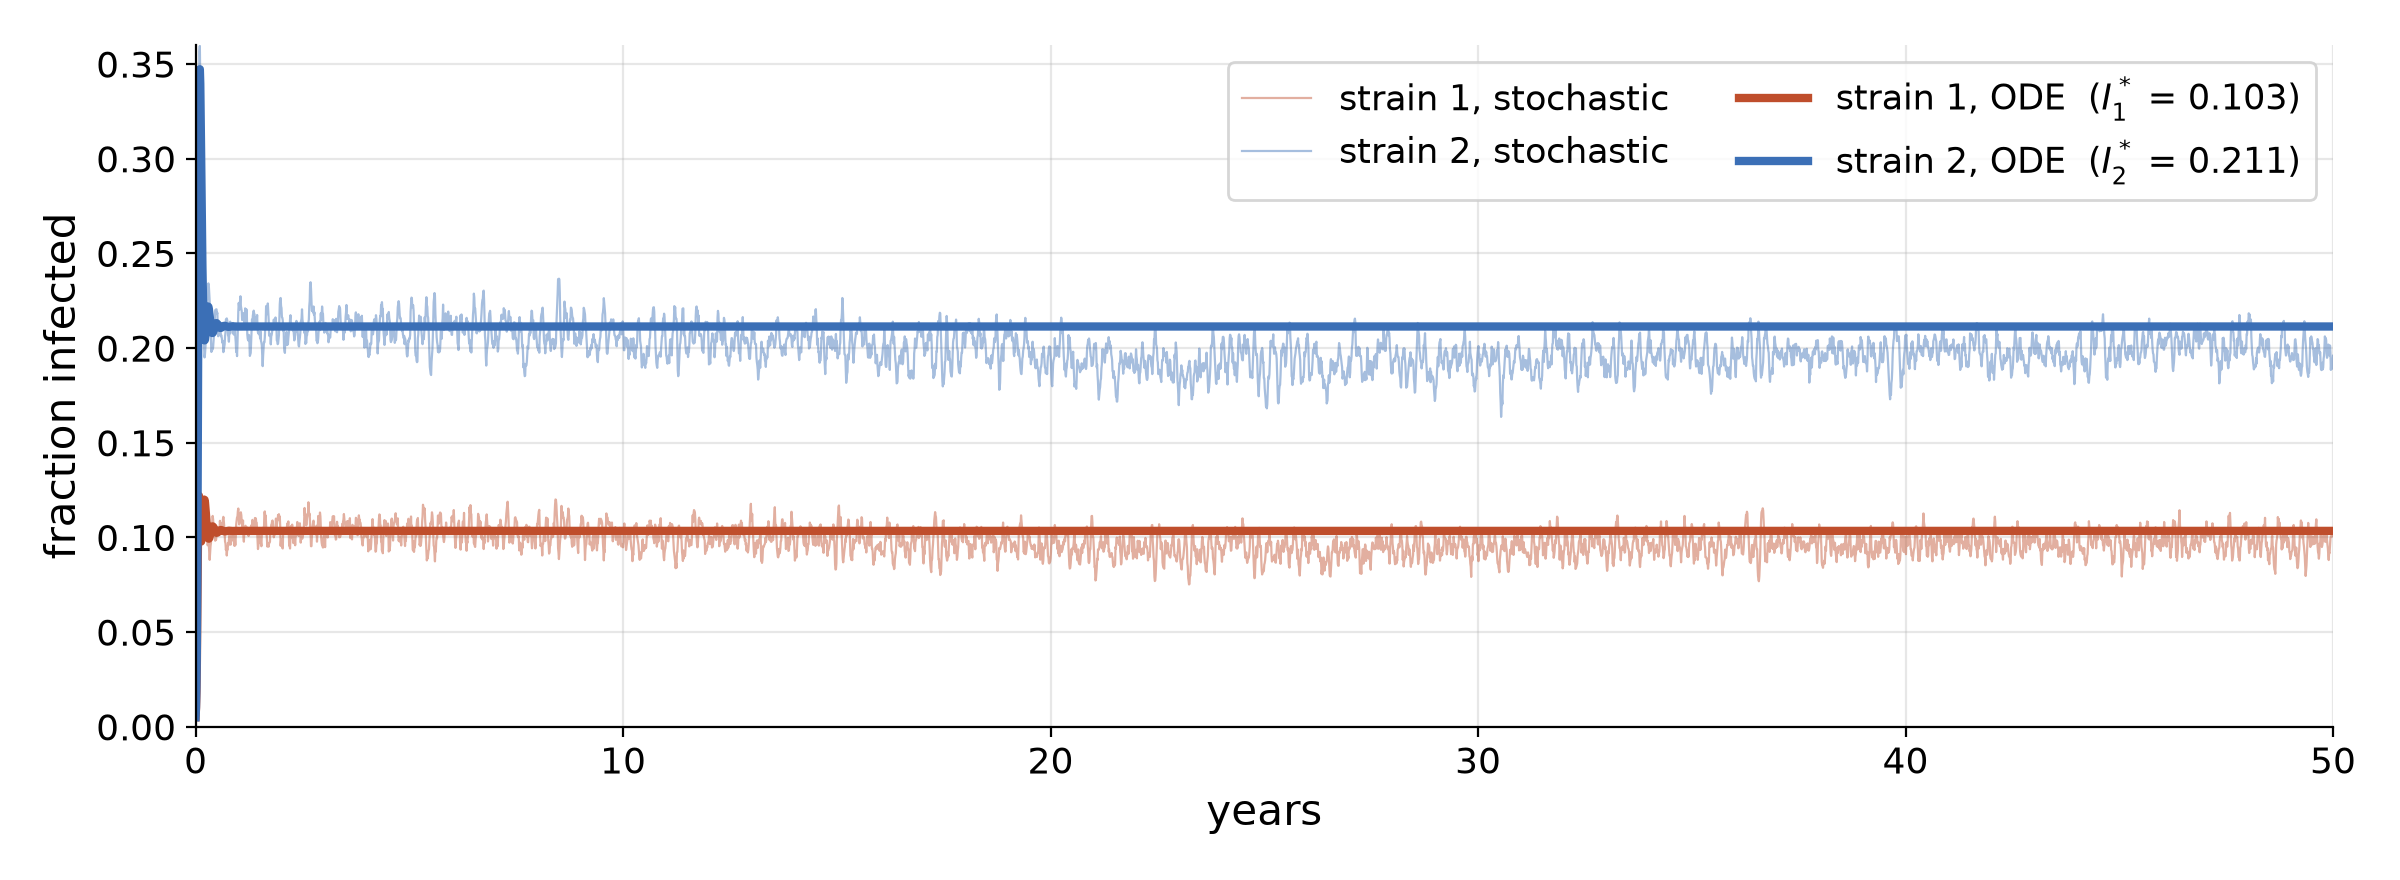
\includegraphics[width=\textwidth]{img/slide_p2_coexistence.png}
\caption{Fraction infected, 50 years. Thick lines: ODE. Thin lines: one SSA run with $N=10{,}000$.}
\end{figure}

\begin{itemize}
  \item After an overshoot in the first month (peaks near $0.12$ for strain 1 and $0.35$ for strain 2) both models settle. The SSA fluctuates around the ODE levels (standard deviations about $0.006$ and $0.009$); the mean over years 10 to 50 is $0.096$ and $0.197$ in this run, against $0.103$ and $0.211$ for the ODE.
  \item The mean level changes by a few percent from run to run ($0.0997$ to $0.1046$ for strain 1 over four other runs of 20 years). In the SSA births and deaths are separate random events, so the total population is not fixed: in the 50 year run it varied between $9{,}686$ and $10{,}031$ (the ODE conserves the total exactly).
  \item \textbf{Check of the code.} The sheet's SSA function (which stores every event and is slow) and the faster implementation used for 50 years (same events, propensities and sampling rule) agree with each other and with the ODE on the mean state after half a year at $N=1000$: for example $I_1=100.8$, $102.5$ and $102.4$ people.
  \item No strain goes extinct in 50 years at this population size.
\end{itemize}

% ======================================================================
\section{Stochastic extinction versus deterministic permanence}\label{sec:zero}

\subsection{In the ODE a strain can never reach zero}

Write $\dot I_1=g(t)\,I_1$ with $g(t)=\beta_1(S+R_2)-(\gamma_1+\mu)$. This is linear in $I_1$, so
\[
I_1(t)=I_1(0)\exp\Big(\int_0^t g(s)\,ds\Big)>0\qquad\text{for every finite }t .
\]
An exponential is never zero. The value may become $10^{-6}$ or $10^{-40}$ but stays positive, and when the susceptible pool refills (births, waning), $g(t)$ becomes positive again and $I_1$ grows from that tiny value: this is the \emph{rebound}. The value has no physical meaning when $I_1N<1$: at $N=10{,}000$, a fraction $10^{-6}$ is $0.01$ of a person.

\subsection{In the SSA zero is absorbing}

$I_1$ is an integer. The only events that increase it are $S\to I_1$ (propensity $\beta_1SI_1/N$) and $R_2\to I_1$ (propensity $\beta_1R_2I_1/N$). Both are proportional to $I_1$. At $I_1=0$ both propensities are 0, so
\[
\Pr\big(I_1(t)=0\ \text{for all }t\ge\tau\mid I_1(\tau)=0\big)=1 .
\]
\hl{When the count of strain 1 reaches zero, strain 1 is extinct for ever.} It cannot rebound, even if the ODE predicts a strong resurgence, because there is no immigration and no other source of infection.

\subsection{Why few infected people means a high risk}

Suppose $k$ people carry a strain, with $k$ small so that the susceptible pool is almost unchanged. Each infected person then acts independently as a birth--death process: a new infection at rate $\lambda=\beta_1(S+R_2)/N$ and removal (recovery or death) at rate $\delta=\gamma_1+\mu$. The next event is an infection with probability $\frac{\lambda}{\lambda+\delta}$ (the line of descent is then replaced by two independent lines) or a removal with probability $\frac{\delta}{\lambda+\delta}$. The extinction probability $q$ of the line descending from one person therefore satisfies
\[
q=\frac{\delta}{\lambda+\delta}+\frac{\lambda}{\lambda+\delta}\,q^2 ,
\]
whose roots are $q=1$ and $q=\delta/\lambda$. The extinction probability is the smallest root in $[0,1]$. With the effective reproduction number $\mathcal R_{\rm eff}=\lambda/\delta=\R^1\,(S+R_2)/N$ and $k$ independent lines,
\[
\Pr(\text{extinction}\mid k)=\begin{cases}1,&\mathcal R_{\rm eff}\le1,\\[3pt]\big(1/\mathcal R_{\rm eff}\big)^k,&\mathcal R_{\rm eff}>1.\end{cases}
\]
Two consequences:
\begin{enumerate}
  \item \textbf{After an epidemic peak} the susceptibles are depleted, $\mathcal R_{\rm eff}<1$, infected numbers fall, and if they reach zero before $\mathcal R_{\rm eff}$ rises above 1 again, extinction is certain.
  \item \textbf{Even with $\mathcal R_{\rm eff}>1$} small numbers are fragile. In a fully susceptible population one infected person of strain 1 starts a lasting epidemic with probability only $1-1/2.307=57\%$ (43\% chance of extinction). With 50 initial cases the extinction probability would be $0.4335^{50}\approx7\times10^{-19}$.
\end{enumerate}
The ODE corresponds to $k\to\infty$, where $(1/\mathcal R_{\rm eff})^k\to0$: this is why it never shows extinction.

\begin{figure}[H]
\centering
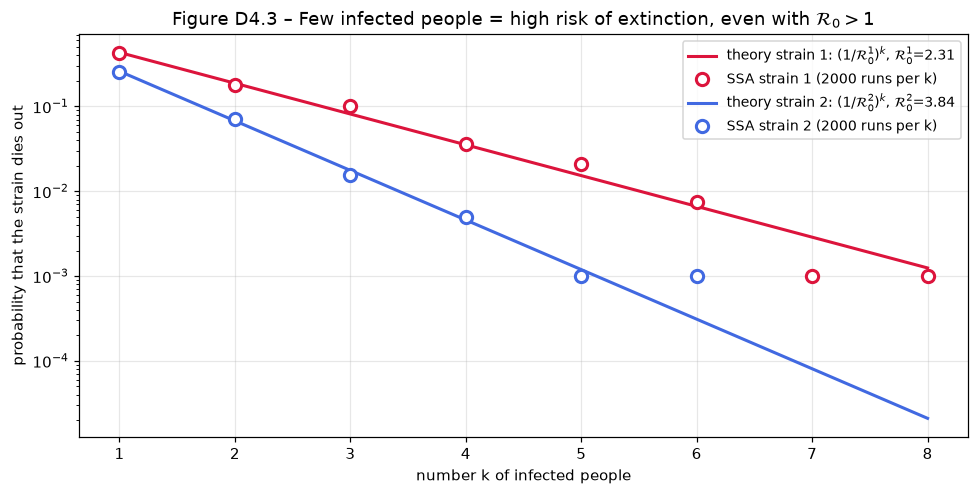
\includegraphics[width=0.78\textwidth]{img/d4_3.png}
\caption{\label{fig:kfig}Probability that a strain started by $k$ infected people dies out before reaching 100 cases ($N=10{,}000$, 2000 simulated runs per point), against the formula $(1/\R)^k$. Points at $10^{-3}$ are one or two events out of 2000 and are at the noise level.}
\end{figure}

\subsection{Results in the model with cross infection}

\textbf{At $N=10{,}000$ there is no bottleneck.} After its first peak (0.123 at $t=0.08$ year), strain 1 goes down to only $0.0977$, that is $977$ people, and settles at its equilibrium ($\approx1030$ people). The same holds for strain 2 (minimum $0.204$ after its peak of $0.347$, about 2000 people). With so many carriers $(1/\mathcal R_{\rm eff})^k$ is negligible and the SSA follows the ODE. So with these parameters the picture of a strain dropping to $10^{-6}$ does \emph{not} occur in the full model at $N=10{,}000$.

\textbf{Smaller populations.} For each $N$ we ran 40 SSA simulations of 50 years, starting with $0.5\%$ of the population infected with each strain (at least one person):

\begin{table}[H]
\centering\small
\renewcommand{\arraystretch}{1.2}
\begin{tabular}{rcccccc}
\rowcolor{aimsred}\color{white}$N$ & \color{white}start per strain & \color{white}ODE $I_1^*,I_2^*$ (people) & \color{white}P(strain lost by year 50) & \color{white}lost in year 1 & \color{white}lost after year 1\\
100 & 1 & 10, 21 & 1.00 & 1.00 & 0.00\\
\rowcolor{rowpink}200 & 1 & 21, 42 & 1.00 & 0.70 & 0.30\\
400 & 2 & 41, 85 & 0.60 & 0.30 & 0.30\\
\rowcolor{rowpink}700 & 4 & 72, 148 & 0.08 & 0.08 & 0.00\\
1000 & 5 & 103, 211 & 0.02 & 0.02 & 0.00\\
10{,}000 & 50 & 1034, 2113 & 0 (single 50 year run) & -- & --
\end{tabular}
\caption{Extinction in the full model. Strain 1 and strain 2 have the same extinction fraction in every row. With 40 runs per $N$, a fraction has a sampling error of up to about 8 percentage points.}
\end{table}

\begin{figure}[H]
\centering
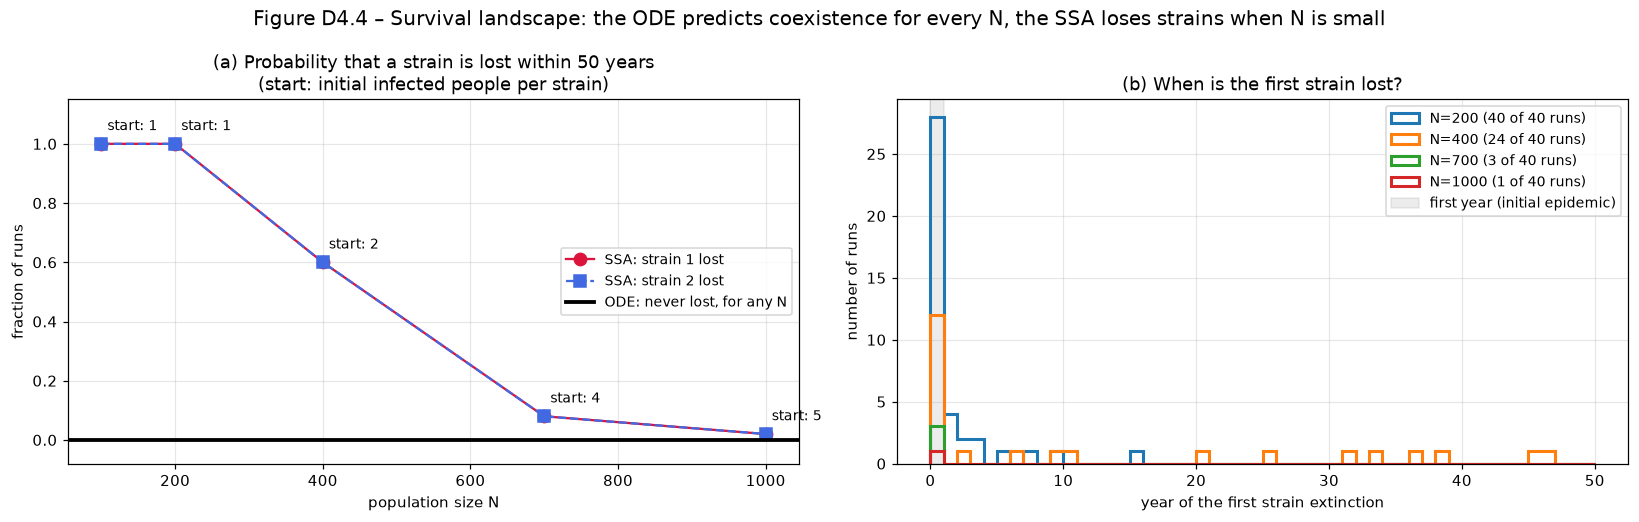
\includegraphics[width=\textwidth]{img/d4_4.png}
\caption{Left: probability that a strain is lost within 50 years as a function of $N$ (the ODE: never, for any $N$). Right: year of the first loss.}
\end{figure}

\begin{itemize}
  \item For $N\ge700$ every loss happens in the first year, when only 4 to 5 people carry each strain (Figure~\ref{fig:kfig} explains why). For smaller $N$ losses also happen later, through random fluctuations around a small equilibrium.
  \item \textbf{The two strains are lost together:} in every row the two strains have the same extinction fraction, and in the example run below ($N=300$) they vanish within a quarter of a year of each other. A plausible reason is that alone each strain is sustained at a much lower level ($0.0024$ and $0.0145$) than in coexistence ($0.103$ and $0.211$), so when one is lost the other is left with very few carriers. We did not test this mechanism separately.
\end{itemize}

\begin{figure}[H]
\centering
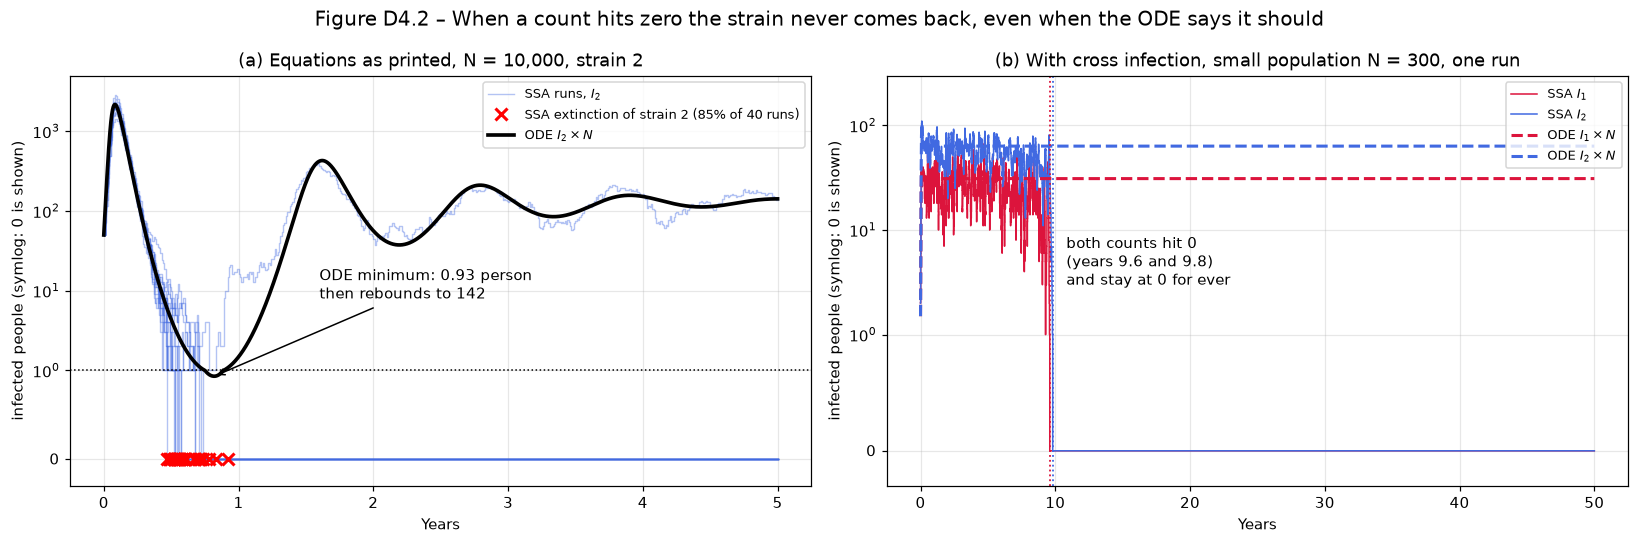
\includegraphics[width=\textwidth]{img/d4_2.png}
\caption{Left: the equations as printed (Section~\ref{sec:printed}), strain 2, $N=10{,}000$: the ODE rebounds, the SSA stays at zero. Right: full model, $N=300$, one run: both strains reach 0 (years 9.6 and 9.8) and stay there, although the ODE predicts $31$ and $63$ infected people for ever.}
\end{figure}

% ======================================================================
\section{The variant: the equations exactly as printed}\label{sec:printed}

Without the cross infection terms the model is
\[
\dot I_i=\beta_iSI_i-(\gamma_i+\mu)I_i,\quad \dot R_i=\gamma_iI_i-(\omega_i+\mu)R_i,\quad \dot S=\mu(1-S)-\beta_1SI_1-\beta_2SI_2+\omega_1R_1+\omega_2R_2 .
\]
The reduction of Section~\ref{sec:reduction} is the same substitution $S=1-I_1-I_2-R_1-R_2$, but the $R$ terms no longer cancel: $\dot I_i=\beta_i(1-I_1-I_2-R_1-R_2)I_i-(\gamma_i+\mu)I_i$ and $\dot R_i=\gamma_iI_i-(\omega_i+\mu)R_i$. The DFE and $\R^i$ are unchanged (they do not depend on the cross infection).

\textbf{No coexistence.} If $I_1^*,I_2^*>0$, then $\dot I_1=\dot I_2=0$ would require $S^*=1/\R^1$ and $S^*=1/\R^2$ at the same time. This is impossible since $\R^1\ne\R^2$. The strain with the larger $\R$ wins (\emph{competitive exclusion}): strain 2 alone settles at $S^*=0.2602$, $I_2^*=0.0145$, $R_2^*=0.7253$. Strain 1 cannot invade it, because its growth rate there is $\beta_1S^*-(\gamma_1+\mu)=120\times0.2602-52.02=-20.8<0$ (the invasion number is $\R^1/\R^2=0.60<1$); this is one of the Jacobian eigenvalues, the others being $-0.99\pm6.12i$ and $-0.22$, so this equilibrium is stable. The ODE reaches it, with $I_1\to0$.

\textbf{This is where the ``tiny value, then rebound'' picture appears.}
\begin{itemize}
  \item ODE, strain 2: peak $0.217$ at $t=0.08$ year, then a fall to $9.35\times10^{-5}$ at $t=0.82$ year, that is \emph{$0.93$ of a person} at $N=10{,}000$, then a rebound to $142$ people by year 5 (the equilibrium is $145$).
  \item ODE, strain 1: $6.8\times10^{-10}$ of a person at year 1, then smaller and smaller, never zero.
  \item SSA, 40 runs of 5 years: strain 1 was lost in 100\% of the runs (within about $0.25$ year) and strain 2 in 85\% (median $0.57$ year, during the trough). Only 6 runs of 40 still had strain 2 at year 5, against $142$ people in the ODE.
\end{itemize}
A dip that the ODE survives is a permanent extinction in the stochastic model.

\begin{figure}[H]
\centering
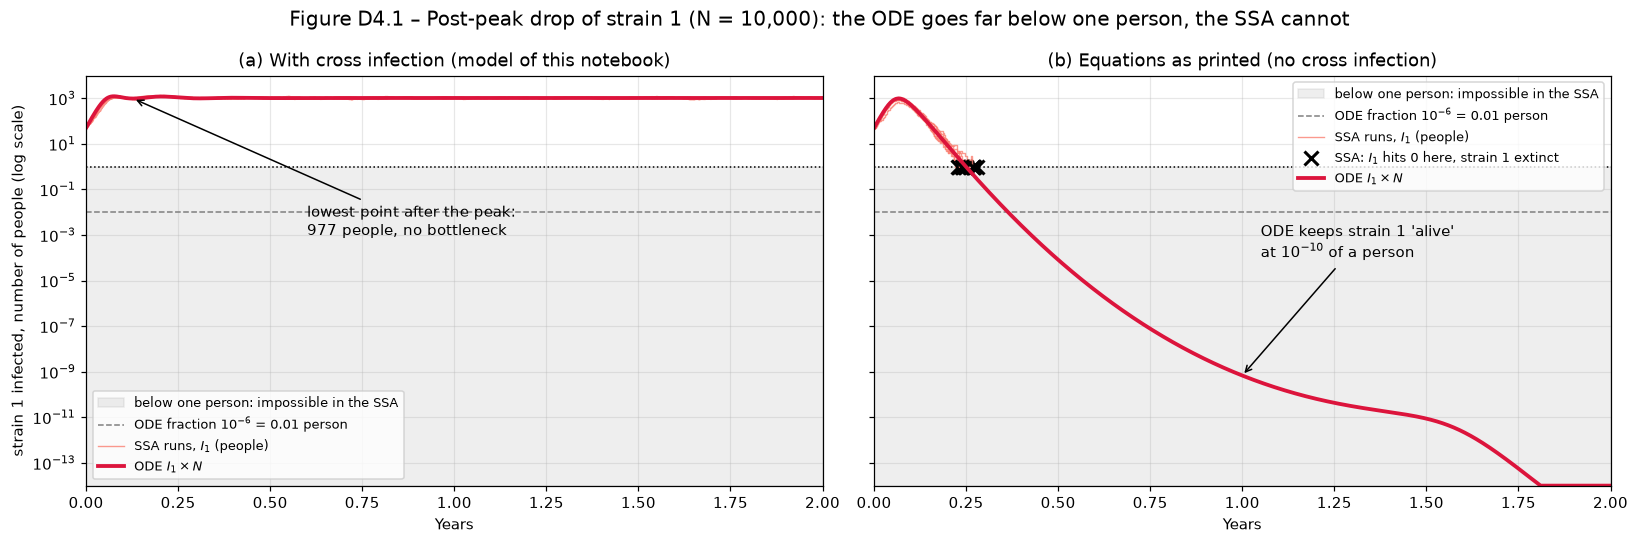
\includegraphics[width=\textwidth]{img/d4_1.png}
\caption{Strain 1 after its peak, in people ($N=10{,}000$, log scale). (a) Full model: shallow drop, lowest point $977$ people, no bottleneck. (b) Printed equations: the ODE goes through ``less than one person'' and passes $10^{-6}$ (0.01 person), and every SSA run reaches 0 (crosses) between years $0.23$ and $0.28$.}
\end{figure}

% ======================================================================
\section{Discussion}

\textbf{What the stochastic bottleneck changes.}
\begin{itemize}
  \item \emph{Deterministic model:} survival is decided only by thresholds ($\R$, invasion numbers), and it does not depend on $N$. In the full model both strains coexist for every $N$; in the printed model strain 2 always wins. A strain can only become small, never disappear.
  \item \emph{Stochastic model:} survival is decided by the number of people $k$ who carry the strain at its lowest point, $\approx N\min_tI_i(t)$, with extinction risk $(1/\mathcal R_{\rm eff})^k$ and $1$ when $\mathcal R_{\rm eff}<1$ for long enough. Because this number scales with $N$, small populations lose strains that the ODE says persist.
  \item Extinction is irreversible. Which strain is lost, and when, is partly a matter of chance (it is not always the one with the lower $\R$), and a lost strain cannot return without reintroduction, although the invasion numbers say it would spread again.
  \item The ODE prediction is trustworthy when $N\min_t I_i(t)\gg1$.
\end{itemize}

\textbf{Limits of this study.}
\begin{itemize}
  \item The extinction formula $(1/\mathcal R_{\rm eff})^k$ treats the carriers as independent and the susceptible pool as constant. It agrees with the simulations for $k\le 6$ (Figure~\ref{fig:kfig}), but it is an approximation.
  \item The stability analysis of the coexistence equilibrium is local. Convergence from the initial condition used was checked numerically over 50 years; global stability was not proved.
  \item The extinction tables use 40 runs per $N$ (Part 2) and 500 runs per $N$ (Part 1), so fractions carry sampling error; $N=10{,}000$ was checked with a single 50 year run and with 40 runs of five years in the printed model. The mechanism by which the two strains are lost together was not tested separately.
  \item In the SSA the total population fluctuates by about 1\% around $N$ (independent births and deaths), whereas the ODE conserves it.
\end{itemize}

% ======================================================================
\section{Conclusion}

\begin{itemize}
  \item For one strain with waning immunity, the ODE predicts an endemic state for $N>\gamma/\beta=15$. The stochastic model adds a new outcome, \hl{stochastic extinction}, even when $\R>1$: in a small population few people are infected, and zero is final. When the infection survives, its average level agrees with the ODE.
  \item For two strains with cross infection, the ODE predicts a stable coexistence ($\R^1=2.31$, $\R^2=3.84$, damped oscillations, no sustained cycles). The stochastic model agrees for $N=10{,}000$, but for small populations both strains are lost. Without cross infection, strain 2 excludes strain 1, and the sharp dip of strain 2 becomes an extinction in 85\% of the runs.
  \item The two descriptions differ at zero: the ODE keeps every positive value alive, the SSA does not.
\end{itemize}

\key{\textbf{Deterministic models describe the large population limit. Stochastic models tell us whether a disease, or a strain, actually survives.}}

% ======================================================================
\appendix
\section{Reproducing the results}

\begin{itemize}
  \item Part 1: notebook \texttt{Project3\_Part1\_SIRS\_SSA\_vs\_ODE.ipynb} (500 runs per $N$, seed $=N$).
  \item Part 2: the ``backup full model'' notebook of Part 2 (model with cross infection; section B: reduction, section D: reproduction numbers, equilibrium, invasion, and Figures D4.1 to D4.4).
  \item ODE: LSODA with relative tolerance $10^{-10}$ and a very small absolute tolerance, so that tiny values are followed. SSA: direct method, fixed random seeds.
  \item Slides: the \texttt{beamer} folder, file \texttt{Project3\_presentation.pdf}. The slide figures are produced by the Python script in the same folder.
\end{itemize}

\end{document}
